% Template for Elsevier CRC journal article
% version 1.2 dated 17 May 2021

% This file (c) 2009-2021 Elsevier Ltd.  Modifications may be freely made,
% provided the edited file is saved under a different name

% This file contains modifications for Transportation Research Procedia

% Changes since version 1.1
% - added "procedia" option compliant with ecrc.sty version 1.2a
%   (makes the layout approximately the same as the Word CRC template)
% - added example for generating copyright line in abstract

%-----------------------------------------------------------------------------------

%% This template uses the elsarticle.cls document class and the extension package ecrc.sty
%% For full documentation on usage of elsarticle.cls, consult the documentation "elsdoc.pdf"
%% Further resources available at http://www.elsevier.com/latex

%-----------------------------------------------------------------------------------

%%%%%%%%%%%%%%%%%%%%%%%%%%%%%%%%%%%%%%%%%%%%%%%%%%%%%%%%%%%%%%
%%%%%%%%%%%%%%%%%%%%%%%%%%%%%%%%%%%%%%%%%%%%%%%%%%%%%%%%%%%%%%
%%                                                          %%
%% Important note on usage                                  %%
%% -----------------------                                  %%
%% This file should normally be compiled with PDFLaTeX      %%
%% Using standard LaTeX should work but may produce clashes %%
%%                                                          %%
%%%%%%%%%%%%%%%%%%%%%%%%%%%%%%%%%%%%%%%%%%%%%%%%%%%%%%%%%%%%%%
%%%%%%%%%%%%%%%%%%%%%%%%%%%%%%%%%%%%%%%%%%%%%%%%%%%%%%%%%%%%%%

%% The ’3p’ and ’times’ class options of elsarticle are used for Elsevier CRC
%% The ’procedia’ option causes ecrc to approximate to the Word template
\documentclass[5p,times,procedia]{elsarticle}
\flushbottom

%% The `ecrc’ package must be called to make the CRC functionality available
\usepackage{ecrc}
%\usepackage{amsmath}


%% The ecrc package defines commands needed for running heads and logos.
%% For running heads, you can set the journal name, the volume, the starting page and the authors

%% set the volume if you know. Otherwise `00’
\volume{00}

%% set the starting page if not 1
\firstpage{1}

%% Give the name of the journal
\journalname{Procedia CIRP}

%% Give the author list to appear in the running head
%% Example \runauth{C.V. Radhakrishnan et al.}
\runauth{B. Bertschinger et al.}

%% The choice of journal logo is determined by the \jid and \jnltitlelogo commands.
%% A user-supplied logo with the name <\jid>logo.pdf will be inserted if present.
%% e.g. if \jid{yspmi} the system will look for a file yspmilogo.pdf
%% Otherwise the content of \jnltitlelogo will be set between horizontal lines as a default logo

%% Give the abbreviation of the Journal.
\jid{trpro}

%% Give a short journal name for the dummy logo (if needed)
%\jnltitlelogo{Transportation Research}

%% Hereafter the template follows `elsarticle’.
%% For more details see the existing template files elsarticle-template-harv.tex and elsarticle-template-num.tex.

%% Elsevier CRC generally uses a numbered reference style
%% For this, the conventions of elsarticle-template-num.tex should be followed (included below)
%% If using BibTeX, use the style file elsarticle-num.bst

%% End of ecrc-specific commands
%%%%%%%%%%%%%%%%%%%%%%%%%%%%%%%%%%%%%%%%%%%%%%%%%%%%%%%%%%%%%%%%%%%%%%%%%%

%% The amssymb package provides various useful mathematical symbols

\usepackage{amssymb}
%% The amsthm package provides extended theorem environments
%% \usepackage{amsthm}

%% The lineno packages adds line numbers. Start line numbering with
%% \begin{linenumbers}, end it with \end{linenumbers}. Or switch it on
%% for the whole article with \linenumbers after \end{frontmatter}.
%% \usepackage{lineno}

%% natbib.sty is loaded by default. However, natbib options can be
%% provided with \biboptions{...} command. Following options are
%% valid:

%%   round  -  round parentheses are used (default)
%%   square -  square brackets are used   [option]
%%   curly  -  curly braces are used      {option}
%%   angle  -  angle brackets are used    <option>
%%   semicolon  -  multiple citations separated by semi-colon
%%   colon  - same as semicolon, an earlier confusion
%%   comma  -  separated by comma
%%   numbers-  selects numerical citations
%%   super  -  numerical citations as superscripts
%%   sort   -  sorts multiple citations according to order in ref. list
%%   sort&compress   -  like sort, but also compresses numerical citations
%%   compress - compresses without sorting
%%
%\biboptions{authoryear}

% \biboptions{}

% if you have landscape tables
\usepackage[figuresright]{rotating}
%\usepackage{harvard}
% put your own definitions here:x
%   \newcommand{\cZ}{\cal{Z}}
%   \newtheorem{def}{Definition}[section]
%   ...

% add words to TeX’s hyphenation exception list
%\hyphenation{author another created financial paper re-commend-ed Post-Script}

% declarations for front matter

\usepackage[bookmarks=false]{hyperref}
\hypersetup{colorlinks,
linkcolor=blue,
citecolor=blue,
urlcolor=blue}

\usepackage{enumitem}
\usepackage{amsmath}
\usepackage{subcaption}
\usepackage{tikz}
\usepackage{relsize}
\usepackage{lipsum}
\usepackage{ulem}

\newcommand{\rem}[1]{\textcolor{red}{\sout{#1}}}
\newcommand{\prop}[1]{\textcolor{blue}{#1}}
\newcommand{\note}[1]{\textcolor{teal}{#1}}

\AtBeginDocument{%
\addtolength\abovedisplayskip{-1.5\baselineskip}%
\addtolength\belowdisplayskip{-1.5\baselineskip}%
\addtolength\abovedisplayshortskip{-2.5\baselineskip}%
\addtolength\belowdisplayshortskip{-1.5\baselineskip}%
%\setlength{\textfloatsep}{1pt }
\setlength{\abovecaptionskip}{0.5\baselineskip} 
\setlength{\belowcaptionskip}{-0.5\baselineskip} 
}

% figures
\usepackage{tikz}
\usepackage{tikzscale}
\usepackage{pgf}
\usepackage{pgfplots}
\usepackage{pgfplotstable}
\pgfplotsset{compat=newest}
\usepackage{float}

\usetikzlibrary{calc,
%	external,
pgfplots.units,
%	pgfplots.external,
pgfplots.groupplots,
arrows,
intersections,
patterns,
positioning,
shapes,
plotmarks,
decorations.pathmorphing,
decorations.markings
}

\hyphenation{metro-logical}
\hyphenation{manu-facturing}

\begin{document}
\begin{frontmatter}
	\dochead{18th CIRP Conference on Intelligent Computation in Manufacturing Engineering}
%
	\title{A new Software Driven External Sensor System for Industrial Robots}
%	
	\author[a]{Bernd Bertschinger\corref{*}}
	\author[b]{Kathrin Hoffmann}
	\author[c]{Jan Baumgärtner}
	\author[b]{Gajanan Kanagalingam}
	\author[c]{Jürgen Fleischer}
	\author[b]{Oliver Sawodny}
	\author[a]{Stephan Reichelt}
	%\ead{author@institute.xxx}
	%
	\address[a]{Institute of Applied Optics, University of Stuttgart - ITO, Pfaffenwaldring 9, 70569 Stuttgart, Germany}
	\address[b]{Institute for System Dynamics, University of Stuttgart - ISYS, Waldburgstr. 17/19, 70563 Stuttgart, Germany}
	\address[c]{Institute of Production Science, Karlsruhe Institute of Technology - WBK, Kaiserstraße 12, 76131 Karlsruhe, Germany}
	%
	\aucores{* Bernd Bertschinger, Tel.: +49-711-685-69892. {\it E-mail address:} bernd.bertschinger@ito.uni-stuttgart.de}
	
	\begin{abstract}
		For decades, laser tracker and total stations have been the state of the art to measure externally the position disturbances in robotic systems. High system costs limit their usage for control systems in common production machines. We present details for an alternative software-driven approach.
		First, we derive a metrological error model for a new self-referencing, high-precision photogrammetry sensor system. Second, we propose a heuristic software approach, which combines an optical simulation pipeline, with motion planning and camera placement to achieve the best possible accuracy. Finally, we outline the hardware implementation and integration in a closed loop control system.
	\end{abstract}
	
	\begin{keyword}
		Photogrammetry \sep Diffractive Optical Element \sep Error Analysis \sep Camera Placement \sep Robot Cell Optimization   \sep	Motion Planing \sep Control Applications
	\end{keyword}
\end{frontmatter}
%
\section{Introduction}
%
Social and ecological changes, as well as the need for
highly individualized and diversified product ranges
motivate not only to increase the efficiency of the means
of production, but also their flexibility of application.
This is addressed by the concept of Wertstromkinematik \cite{Muehlbeier2020}. Herein, the factory is not a static setup to produce one set of goods, but can be dynamically reconfigured to be a generalized production floor. This need for flexibility leads to an increase of precision, which can be used to either facilitate the production of high-precision components, for human-robot and robot-robot collaboration, as well as a trade-off for higher process speed.\\
At the current state of the technology, robotic systems use internal sensors, which require an exceeding level of mechanical stiffness. An alternative are external sensors, such as laser trackers and total stations \cite{Moeller17, Yang17}. The costs of these systems make them unsuitable for widespread production applications. This leads to a dilemma between acquisition costs and system flexibility. To overcome this a holistic approach is chosen, as detailed below.
%
%
\subsection{Scope of this Paper}
The first section \textit{Process Perception} introduces a camera sensor with increased 2D resolution, which facilitates the need for a universal \textit{Metrological Error Model} to assess the probability of detection in a multi camera setup, based on the fusion of stereoscopic sub-sensors and the corresponding confidence ellipsoid. To \textit{Optimize Perception} it becomes mandatory to determine the covariance of triangulation, for which a new optical simulation pipeline is introduced.\\
On this basis, a distinct optimization criterion for the subsequent section \textit{Process Strategies} is derived. Here we define a motion planning procedure to be extended by the metrological error model. The \textit{Hardware Implementation}  is introduced, which is composed of an external sensor system and robot and will be used for validation. Based on a \textit{Kinematic Strategies} analysis, we assess ways to consider geometric errors and offline calibration techniques to be suffice for the initial \textit{Path Planning}. Based on the previous works, we introduce a second robot to segment the path in a 4-step process.\\
While the previous steps have minimized the error in the task space, forces and torques lead to undesirable errors in the joint space.
Hence, \textit{Dynamic Strategies} for compensation are evaluated, and a predictive model is introduced to trade-off process speed and accuracy. For the \textit{Trajectory Generation} a solution for the optimal control problem is introduced that minimizes travel time. The Solution can be extended to improve the accuracy by the aforementioned dynamic data-driven error model and the metrological covariance analysis.\\
The trajectory is the final key-stone for the \textit{Camera Placement}. Here, we finalize the set-up and determine the camera positions to minimize obscurance and maximize accuracy.
%
\section{Process Perception}
%
Recent research indicates that multipoint photogrammetry might be a solution to realize cost-efficient high-resolution optical sensors \cite{Hartlieb_2021}.
The schematics of this measuring method is shown in Fig.~\ref{fig:MeasSys_Errors}.
\begin{figure}[h]
	\centering
	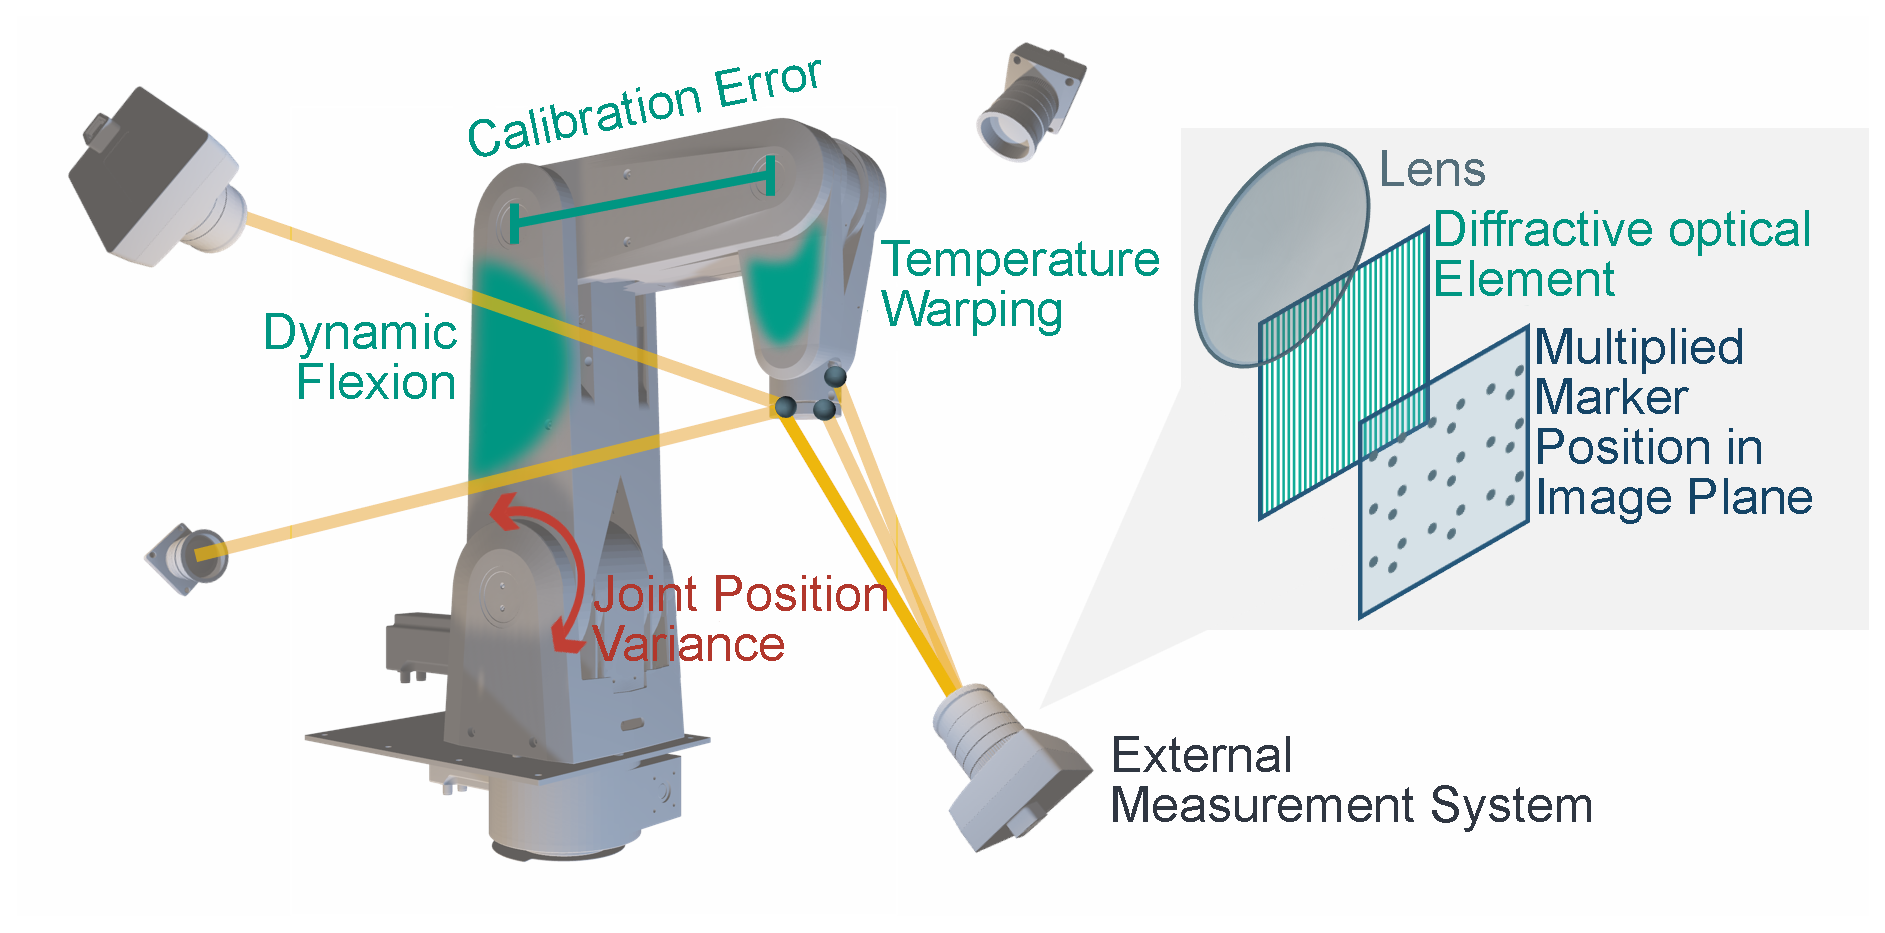
\includegraphics[width=1.0\columnwidth]{graphics/error_sources.eps}
	\caption{Error sources in a robotic manufacturing system, which can be compensated using an external multipoint  sensor, are marked in green.}
	\label{fig:MeasSys_Errors}
\end{figure}
In this method, a Diffractive Optical Element (DOE) is used in succession of an imaging lens to create multiple linearly independent optical copies of an active marker.
It has been shown \cite{Hartlieb_2021} that the variance of the mean positional detection error of these points $\sigma_{x’y’}^2$ detected on the imaging sensor is proportional to the number of copies $n_{pt}$ created by the DOE.\\
However, this increase in planar signal detection is in itself not sufficient for high precision 3D localization. One or more additional sensors are needed to triangulate the 2D point positions on the imaging sensors to its point of origin in the object space. \\
For a pinhole camera system the relation between object and imaging point is determined by the camera matrix $\mathbf{C}$, which is composed of the intrinsic $\mathbf{K}$ and  and extrinsic camera parameters $[\mathbf{R}, \mathbf{t}]$, which comprise information about the spatial orientation, as well as the information about distance to image plane and
image scale factor. This leads to the well established collinear equation \cite{Luhmann2003}, whereby $l_n$ is the collinear factor, which describes the line of sight between the object and image point.
%
\begin{align}
	\mathbf{C} = \mathbf{K}
	\begin{bmatrix}
		\mathbf{R} & \mathbf{t} \\
		0 & 1 \\
	\end{bmatrix} \\
	l_{n}
	\begin{bmatrix}
		x_n’ \\
		y_n’ \\
		0
	\end{bmatrix}
	= \mathbf{C}
	\begin{bmatrix}
		x \\
		y \\
		z \\
		0
	\end{bmatrix}
\end{align}
%
Subsequently, the correspondence between object position and image points, known as triangulation, can be defined for multiple cameras according to:
%
\begin{equation}
	\label{eqn:triangulation}
	\begin{bmatrix}
		x_{1}’ \mathbf{C}_{3,1}^{\top} - \mathbf{C}_{1,1}^{\top}\\
		y_{1}’ \mathbf{C}_{3,1}^{\top} - \mathbf{C}_{2,1}^{\top}\\
		x_{2}’ \mathbf{C}_{3,2}^{\top} - \mathbf{C}_{1,2}^{\top}\\
		y_{2}’ \mathbf{C}_{3,2}^{\top} - \mathbf{C}_{2,2}^{\top}\\
		\vdots \\
		x_{n}’ \mathbf{C}_{3,n}^{\top} - \mathbf{C}_{1,n}^{\top}\\
		y_{n}’ \mathbf{C}_{3,n}^{\top} - \mathbf{C}_{2,n}^{\top}\\
	\end{bmatrix}
	\begin{bmatrix}
		x \\
		y \\
		z \\
		1
	\end{bmatrix}
	=
	\begin{bmatrix}
		0 \\
		\vdots \\
		0
	\end{bmatrix}
\end{equation}
%
Where $C_{m,n}$ corresponds to the $m$-th row of the $n$-th camera matrix.
In case the extrinsic and intrinsic camera parameters are fully known, the equation system can be solved by least-square techniques \cite{Ahn2004}.\\
It is important to note that this relationship can also be described by the notation for projective reconstruction \cite{Hartley2018}:\\
%
\begin{equation}
	\label{eqn:ProjectiveReconstruction}
	x’^{\top}\mathbf{F}x
\end{equation}
%
Here, the fundamental matrix $\mathbf{F}$ is a $3\times 3$ tensor, which scales in rank according to the number of cameras in the system. Due to the increasing complexity and computing effort, this method is usually constraint to three cameras systems. Instead of a Tensor representation, the triangulation relation (\ref{eqn:triangulation}) is stated in implicit form\\
%
\begin{equation}
	\label{eqn:ImplicitFrom}
	\begin{aligned}
		& g(\mathbf{Q},\mathbf{M}) \\
		& \mathbf{Q} = [\mathbf{P},\mathbf{C}]^{\top}
	\end{aligned}
\end{equation}
%
The vector of the input Quantities $\mathbf{Q} = \left[q_1,\dots, q_{n}\right]^{\top}$ is composed of the vector of image points $\mathbf{P} = [x’_1,y’_1, \dots ,x’_n,y’_n]^{\top}$ and the vector of camera parameters, $\mathbf{C} = \left[ \mathbf{C}_1 , \dots , \mathbf{C}_n \right]^{\top}$, which in turn define the object point coordinates $\mathbf{M} =  [x,y,z]^{\top}$ in cartesian form. The uncertainty of the output $\mathbf{M}$ can be approximated by the 1st order Taylor series with regard to the input parameters:\\
%
\begin{equation}
	\sigma^2 = \sum_{i=1}^{n}\sum_{j=1}^{n} \left(\frac{\delta g}{\delta q_i}\right) \left(\frac{\delta g}{\delta q_j}\right) \mathrm{cov}(q_i, q_j) 
\end{equation}
%
Where $\mathrm{cov}(q_i, q_j) $ is the covariance between two input parameters. More commonly, it is known in the form~\cite{Cox2006}
%
\begin{equation}
	\sigma^2 = \mathbf{J_{Q}}\mathbf{\Lambda_{Q}}\mathbf{J_{Q}}^{\top}
\end{equation}
%
$\mathbf{J_{Q}}$ is known as design or Jacobi matrix of the partial derivatives of $g\left(\mathbf{Q},\mathbf{M}\right)$ with respect to the input quantities $\mathbf{Q}$, and $\mathbf{\Lambda_Q}$ is the covariance matrix of said input values. The uncertainty of the input parameters is directly tied to the uncertainty of the output parameters\\
%
\begin{equation}
	\mathbf{J_{M}}\mathbf{\Lambda_{M}}\mathbf{J_{M}}^{\top} = \mathbf{J_{Q}}\mathbf{\Lambda_{Q}}\mathbf{J_{Q}}^{\top}
\end{equation}
Therein, $\mathbf{J_{M}}$ is the Jacobi matrix of the partial derivatives input quantities $\mathbf{M}$ and $\mathbf{\Lambda_{M}}$ is the covariance matrix with respect to the output quantities $\mathbf{M}$.
The matrix $\mathbf{\Lambda_{M}}$ is computed as
\begin{equation}
	\mathbf{\Lambda_{M}} = \mathbf{J_{M}^{\Delta}} \left( \mathbf{J_{Q}}\mathbf{\Lambda_{Q}}\mathbf{J_{Q}}^{\top}\right) \left(\mathbf{J_{M}^{\Delta}}\right)^{\top}
\end{equation}
With $ \mathbf{J_{M}^{\Delta}} = \left( \mathbf{J_{M}^{\top}} \mathbf{J_{M}^{}} \right)^{-1}\mathbf{J_{M}^{\top}}$ being the Moore-Penrose pseudo inverse matrix of $\mathbf{J_M}$.
%
\subsection{Metrological Error Model}
\label{met_err_model}
The design matrices for the input $\mathbf{J_{Q}}$ and output quantities $\mathbf{J_{M}}$ can be established by a various calibration processes \cite{Hartley2018}.  A detailed description of these methods exceed the scope of this paper. Usually a series of known markers is placed in the object space \cite{Luhmann2003}. In case of arbitrary camera positions the minimum number of marker needed corresponds to
%
\begin{equation}
	\label{eqn:NumCalibPoints}
	\begin{aligned}
		& 	u = u_n \cdot n_{pictures} + u_p \cdot n_{points} + u_c \cdot n_{cameras} \\
		& \text{with: } u_n = 6\text{, } u_p = 3\text{, } u_c = 6 
	\end{aligned}
\end{equation}
%
Whereby $u_n$,$u_p$,$u_p$ is the minimum number of unknown parameters to be resolved and $n_{pictures}$,$n_{points}$,$n_{cameras}$, is the 
number of pictures, points per picture and cameras within the system. It becomes evident, that an increase in the number of cameras $n_{\text{cameras}}$ leads to increasing requirements for the means of calibration (\ref{eqn:NumCalibPoints}) and computational complexity, signified by the increasing rank of the fundamental matrix (\ref{eqn:ProjectiveReconstruction}). Conversely, it becomes difficult to determine the metrological error of such as system.
%
\begin{figure}[H]
	\centering
	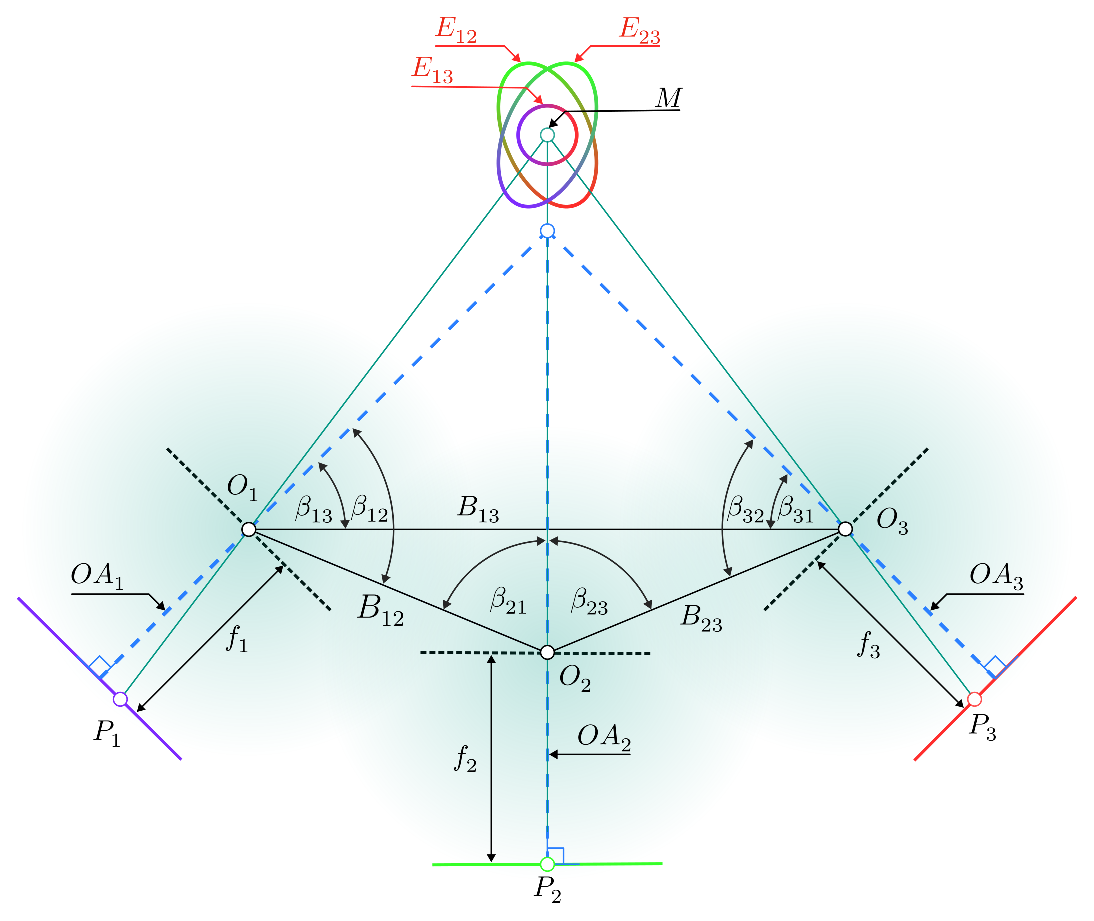
\includegraphics[width=0.90\linewidth]{graphics/MixedErrorCuttingGeometry.eps}
	\caption{Top view of a photogrammetric sensor in trifocal configuration under simplified converging geometric constraints, whereby the optical axes $OA$ of three cameras systems intersect in one point.		
		It can also be regarded as a composition of $n_{sub}=3$ stereoscopic subsystems, whereby the measurement error of each subsystem corresponds in shape to an ellipsoid $\mathbf{E}$.}
	\label{fig:sub_sensors}
\end{figure}
%
Hence, an alternative approach is needed. As depicted in  Fig.~\ref{fig:sub_sensors} a photogrammetric sensor can also be described as a combination of multiple independent stereoscopic sub-sensors.
%
\begin{equation}
	\label{eqn:CovarianceMatrix}
	n_{sub} = \sum_{n=1}^{n_{cam}}n-1
\end{equation}
%
For these subsensors the metrological error can be described as an ellipsoid $\mathbf{E}$ \cite{Luhmann2003}, which is related to a spectral decomposition of the covariance of the output quantities $\mathbf{\Lambda_{M}}$.
%
\begin{equation}
	\mathbf{\Lambda_{M}} =
	\begin{bmatrix}
		\mathbf{S}_1^{} & \mathbf{S}_2^{} & \mathbf{S}_3^{}
	\end{bmatrix}^{\top}
	\begin{bmatrix}
		\lambda_1^{} & 0 \\
		0 & \lambda_2^{} &  0 \\
		0 & 0 &  \lambda_3^{}
	\end{bmatrix}
	\begin{bmatrix}
		\mathbf{S}_1^{} \\
		\mathbf{S}_2^{} \\
		\mathbf{S}_3^{}
	\end{bmatrix}.
\end{equation}
%
The normalized eigenvectors $\mathbf{\hat{S}}_i = \mathbf{S}_i / |\mathbf{S}|$ correspond to the direction of the semi-axis of the ellipsoid and the square root of product of the eigenvalues $\lambda_i$ and the quantile of the $\chi^2_{3,1-\alpha} $ distribution with regard to the probability of safety $1-\alpha$ \cite{Pelzer1995}.
%
\begin{equation}
	\mathbf{E} =
	\begin{bmatrix}
		e_{11}^{} & e_{12}^{} & e_{13}^{} \\
		e_{21}^{} & e_{22}^{} & e_{23}^{} \\
		e_{31}^{} & e_{32}^{} & e_{33}^{}
	\end{bmatrix}
	=
	\sqrt{ \chi^2_{3,1-\alpha}}
	\begin{bmatrix}
		\mathbf{\hat{S}}_1^{} & \mathbf{\hat{S}}_2^{} & \mathbf{\hat{S}}_3^{}
	\end{bmatrix}
	\begin{bmatrix}
		\sqrt{\lambda_1^{}} \\
		\sqrt{\lambda_2^{}} \\
		\sqrt{\lambda_3^{}}
	\end{bmatrix}
\end{equation}
%
Since the angular orientation of the ellipsoids is non-isotropic, the world coordinate system
is defined as frame of reference. Thereby not the semi-axes, but the intersection with the coordinate
axes is used for further computation. Hence, the metrological error along the unit vectors equals
%
\begin{equation}
	\sigma_j = \sum_{j=1}^{3} \left( e_{ij} + e_{ij} + e_{ij}\right)
\end{equation}
%
Subsequently, the metrological error for each subsystem $\sigma_{j,n}$ can be used to combine and improve the related outcomes $\mathbf{M}_n$ by calculating the weighted arithmetic mean \cite{Price1972}
\begin{equation}
	\mathbf{\bar{M}}_{j} = \frac{\sum_{n=1}^{n_{sub}} \left( \mathbf{M}_{n,j} \cdot \sigma_{n,j}^{-2} \right)}{\sum_{n=1}^{n_{sub}} \sigma_{n,j}^{-2}}
\end{equation}
The resulting error corresponds to
\begin{equation}
	\mathbf{\bar{\sigma}}_{j} = \sqrt{ \frac{1}{\sum_{n=1}^{n_{sub}} \sigma_{n,j}^{-2}} }.
	\label{eqn:sum_noise}
\end{equation}
%
\subsection{Optimized Perception}\label{subsec:OptPerception}
It has been remarked in the literature~\cite{Di_Leo_2011} that a covariance exists between the input quantities of a stereoscopic system, and it is related to a combination of marker and the image processing algorithm used for detection.
Only recently, for the case of a simplified stereoscopic sensor under converging constraints and passive markers, simulation results have experimentally been verified.\\
Liu et al.~\cite{Liu_2021} showed that the optimum camera orientation angle $\beta_{mn}$ is in the range of $60^{\circ} -\, 80^{\circ}$, not $30^{\circ} \text{-}\, 50^{\circ}$ \cite{Yang2018,Fooladgar2013,Sankowski2017}. The input quantities for such a system are depicted in Fig.~\ref{fig:sub_sensors} and read
%
\begin{equation*}
	\mathbf{Q}= \left[x’_m, y’_m, x’_n, y’_n, \beta_{mn}, \beta_{nm}, B_{nm}, f_{n},f_{m}\right]^{\top}
\end{equation*}
%
In this case $x’, y’$ is the pixel position of the marker on the sensor plane, $\beta$ is the aforementioned camera orientation angle, $B$ is the distance between the pinhole position and $f$ is the focal length.\\
The off-diagonal elements of the resulting covariance matrix $\mathbf{\Lambda_{Q}}$ signify high degrees of cross-correlation between the camera orientation angle $\beta$ and the point position $x,y$ on the detector. This is related to the decreasing visible surface of the passive markers, which leads to an increase of the effective noise per area.\\
Since multipoint detection \cite{Haist2015} uses sub-resolution active markers instead of passive ones, it cannot be assumed that the cross-correlation factors are similar. Since here, the so-called signal-to-noise ratio (SNR) primarily depends on intensity of the spots on the sensor plane.
%
\begin{figure}[!htb]
	\centering
	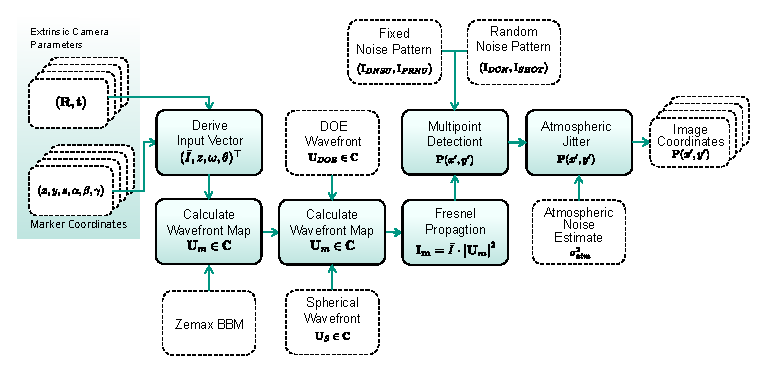
\includegraphics[width=1.0\columnwidth]{graphics/OpticalSimulation.eps}
	\caption{Simulation procedure for multipoint detection based on a black-box-model (BBM) and a combination of geometric and Fresnel propagation.}
	\label{fig:opto-sim}
\end{figure}
This signal strength is on the one hand related to the distance between sensor and marker \cite{dumbleton1955}, on the other hand it depends on the spatial orientation of the marker with regard to the receiving optic. The radiation characteristic of a LED or a diffuser fiber tip \cite{Pan1994} is for most angular orientations non-isotropic.\\
On this basis an optical simulation procedure was created, as can be seen in Fig.~\ref{fig:opto-sim}, to extended previous works \cite{Liu_2021,Di_Leo_2011} about the covariance-analysis for stereoscopic sensors.\\
Here, the extrinsic camera parameters and the marker coordinates in space and orientation are used to derive
the input vector for the simulation, which comprises information about the normalized intensity distribution $\bar{I}$, the distance to marker $z$ and the field angles $\omega$ and $\theta$. A black box model of the lens is used to compute the complex wavefront distribution at the DOE-position $\mathbf{U}_m$, which is combined with the DOE phase distribution $\mathbf{U}_{DOE}$ and a spherical wavefront $\mathbf{U}_{S}$ to accommodate for the distance of the DOE to the imager. This wavefront is propagated to the sensor by the Fresnel method \cite{Goodman2005}. The fixed $\mathbf{I}_{DNSU/PRNU}$ and random $\mathbf{I}_{DCN/SHOT}$ noise patterns are superimposed onto the derived sensor intensity distribution $\mathbf{I}_m$ and the point coordinates $\mathbf{P}_{x’,y’}$ are derived via multipoint detection.
Finally, the point position is varied by an estimate of the atmospheric disturbance.\\
As can be seen from Eq.~\ref{eqn:sum_noise}, one can state that more cameras lead to a smaller metrological error.
However, the restriction is  that they need to be placed such that they can perceive the target at all -- only then an increase of in the number of cameras used lead to an improved perception.\\
Therefore, a strategy to place the cameras is presented in the later part of the next section.
%
\section{Process Strategies}
Besides the aforementioned placement of the cameras, incorporating the metrological error estimate as referenced in section \ref{subsec:OptPerception} also opens up new possibilities for a software-defined motion planning.
To find a compromise between accuracy and speed, the motion planning problem is divided into path planning and path trajectory generation, which is a common approach in the literature~\cite{Choset05}.\\
In path planning, the path of each of the robots' joint angles is computed, providing the highest possible repeatability.
In trajectory generation, the previously computed path is indexed in time so that the robot can follow the given paths as quickly as possible such that the process speed is maximized, taking into account dynamic constraints of the robot (e.g. actuator dynamics).
This also allows for a separate consideration of kinematic and dynamic errors of the robot system. 
Once the configuration of the robot is known from the motion planning steps, also the placement of the cameras for the process perception can be optimized as described in this section as well. 
%
\subsection{Hardware implementation}
The optical measurement system is set up with the trifocal sensor according to section~\ref{met_err_model}.
The camera measurements are processed on a computer, which communicates via a CAN bus with a rapid prototyping system controlling the robot.
This enables synchronized measurements of the camera, joint angles (encoders) and joint torques.
The rapid prototyping system runs an interface through which the reference values for the joint space position, velocity and acceleration are directly communicated to the built-in robot trajectory tracking controller.\\
In the present work, the robot joints are realized as pneumatic direct drives, which has the advantage that the drive angle can be directly measured without backlash. 
The disadvantage, however, is that the drive dynamics are slower than of electric drives. Strong friction effects occur, which means that they have a similar effect on precision as gears in electric drives, so that for both robot types there result dynamic errors in the joint angles. 
%
\subsection{Kinematic strategies}
Some kinematic strategies for increasing the accuracy of industrial robots are already well-established.
Purely geometric errors in a robot can stem from the sources' length deviations of links, axis misalignment and zero-position offsets of the encoders and can be identified and compensated in an offline calibration technique~\cite{Wiest01}.
To this end, the end effector pose is measured with an external measurement statically at certain points in the workspace a certain number of times, and the geometric error parameters are determined in an optimization.
This procedure does not generalize well the entire workspace and can not be used during the industrial robot application itself, but provides a first enhanced kinematic model of the robot.
Such calibration also captures the static deformation of the robot structure, which is however load dependent, so that an a priori calibration measurement may not generalize well. This is another motivation for adding an external optical measurement system during robot operation.
Incorporating the a priori manufacturing tolerances into the forward kinematic model yields an error measure in the task space.
It is reasonable to assume these errors are usually much larger than the accuracy of the presented measurement system. It also captures the static deformation of the robot structure, which cannot be separated under different loads.
%
\subsection{Path Planning}\label{subsec:PathPlanning}
There are several error sources impeding the accuracy of a robotic manufacturing system.
An overview of these sources can be seen in Fig.~\ref{fig:MeasSys_Errors}.
Most of these errors can be captured with the present measurement system and from that be compensated.
This leaves the finite precision of the robot itself, whose contribution can not be compensated but only mitigated.
Previous works such as \cite{previous_work} have shown that the optimal repeatability of a path is dependent on the workpiece placement.\\
This means that we can use a second workpiece holding robot to reposition the workpiece in such a way that the optimal repeatability is achieved. It might be tempting to try to find a continuous trajectory of this second robot to minimize the error. However, this machine also suffers from finite joint precision, while moving these will introduce additional errors.
It is therefore better if the workpiece holding robot moves to a fixed position before the primary robot starts moving \prop{\cite{stroke_division}}. %\rem{
	%This leads to a two-step process similar to the one described in \cite{stroke_division}.}
\prop{\\}
Here, the authors propose a 4-step process to path planning:
\begin{enumerate}
	\setlength\itemsep{-0.5em}
	\item Cut path into multiple segments
	\item Downsample each segment
	\item Optimize the pose of each subpath\\and compute the joint path
	\item Apply the new pose to the original segments
\end{enumerate}
The division of the path into multiple segments was performed by identifying turning points using path simplification algorithms \cite{stroke_division}.
However instead of using the pose optimization algorithm described in \cite{stroke_division} we use the problem formulation of \cite{previous_work} since it allows us to integrate more constraints which are later used for the joint trajectory optimization.
%
\subsection{Dynamic Strategies}\label{subsec:dynError}
In addition to kinematic errors, there occur also dynamic errors resulting from forces and torques in the robotic system.
Resulting trajectory tracking errors can be captured in the optical measurement of the robot end effector, and for example be compensated by a classical task space controller~\cite{Siciliano09}.
Tracking errors are more systematic in joint space than in task space.
In the present robot with direct drives, the joint angle tracking error is directly measured, while for other drive types this can be realized with secondary encoders~\cite{Mesmer22}.\\
In order to not only compensate such errors by feedback but also to take them into account during trajectory generation, a dynamic error model is desirable.
There is a large amount of literature on learning either black-box models~\cite{NguyenTuong08b} or data-driven supplements to parametric models in the form of a gray-box model.
In the following, a dynamic model for the control error of an exemplary drive is introduced.
Since hysteresis occurs in the drives and dynamic effects are to be captured, not only the current position, velocity and acceleration state of the drive but also the motion history several samples back is included. 
To this end, a Gaussian process (GP) dynamic model is set up.
It is trained with desired reference values instead of actual values to be able to predict dynamic errors for given trajectories.
For training, the same path is executed at different speeds. 
The GP is then used to predict the dynamic error when executing the path at other previously unseen velocity profiles.
This dynamic error model can then be incorporated in an optimization to allow for a trade-off between process speed and accuracy.
%
\subsection{Trajectory Generation}
In section~\ref{subsec:PathPlanning} the path has been determined under the premise of optimal repeatability. Hereon, a trajectory is generated to maximize the robot’s travel speed and thus the process time.
To generate the trajectory, the already determined path of all joint angles is parameterized, and thereby all individual paths are implicitly synchronized.
Since the robot applied in this work has the mathematical property of differential flatness~\cite{Hoffmann23}, the state of the robot can be represented with the help of the given trajectory of the individual joint angles, the path parameter and its time derivatives.\\
In order to generate the trajectory, it is now sufficient to determine the time derivatives of the path parameters by means of an optimal control problem. 
Hence, the travel time is minimized, taking into account the dynamic, state-dependent constraints of the robot. For a more detailed description of trajectory generation, please refer to~\cite{Kanagalingam24}.
%
This existing formulation can not only optimize travel time and/or energy efficiency, but also the accuracy.\\
To this end, the data-driven error model from section~\ref{subsec:dynError} can be added to the optimal control problem.
To quantify the errors, the mean value function of the Gaussian process is added while the covariance serves to assess the certainty of the model, which can additionally be included in the cost functional. Therefore, future work will include optimization-based trajectory generation with this data-driven component added to the optimal control problem.
%
\subsection{Camera Placement}
With the robot configuration being known from the previous steps, the perception of the process can be optimized:
After planning the path, the two robots are bound to perform complex movements that might obscure some markers from the camera.
It might even be the case that all markers are visible, but that they are in regions where the camera system has a low measurement accuracy.
\begin{figure}[H]
	\centering
	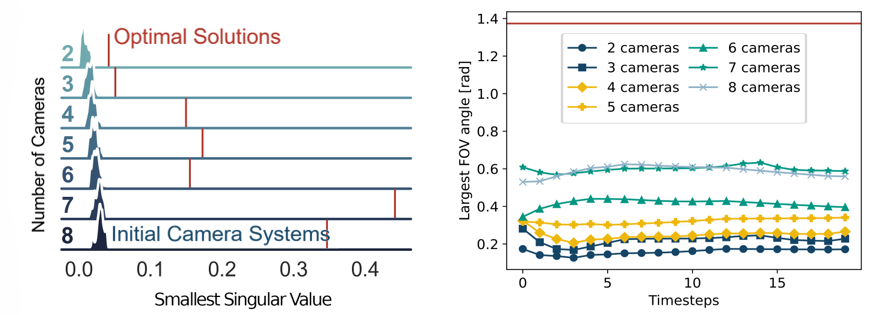
\includegraphics[width=0.95\columnwidth]{graphics/fov_sv_conflict.png}
	\caption{The conflict between the field of view angle and the smallest singular value. Left: The smallest singular values of the system replicated from \cite{camera_placement}. Right: The largest angle of a marker to the optical axis.
		Comparing both, one can see that lower singular values correlate with lower maximum field of view (FOV) angles.}
	\label{fig:fov_sv_conflict}
\end{figure}
To mitigate both problems, we propose a software system that can optimize the placement of the cameras as needed.
This system is largely based on the work of \cite{camera_placement} and follows a two-step optimization approach.
However, instead of only considering the condition of the triangulation equation as well as visibility, we use the full error model described in section \ref{met_err_model}.\\
In this way, the benefits can be weighted against the additional effort required  for repositioning and recalibration.\\
Replicating the results of \cite{camera_placement} where the smallest singular value was used as a measure of the quality of the camera placement, we can additionally plot the largest angle to the optical axis.
Here we see that the system always tries to find a trade-off between minimizing the field of view angle while trying to maximize the smallest singular value.
This is shown in Fig.~\ref{fig:fov_sv_conflict}.
In a unified error description, this problem does not exist, and the system can be optimized for the best possible accuracy.
%
\section{Outlook \& Conclusion}
A new software driven production process has been introduced to facilitate the highest level of manufacturing precision.
Therefore, a metrological error model for a photogrammetric sensor system was presented and kinematic and dynamic strategies
for motion planning were derived. By means of robot-robot collaboration and path segmentation, the kinematic error was minimized. This path was then translated into a trajectory by minimizing the travel time. On the basis of the GP dynamic model and the covariance of triangulation, the system accuracy can be further improved. Finally, a placement strategy based on said trajectory was introduced, which minimizes obscurance and avoids areas of low accuracy. By this means the authors are confident to achieve similar levels of accuracy compared to today's laser tracker and total stations.\\
So far, the introduced optical simulation model has only been verified qualitatively. Though this is a reasonable base for the current state of development, a quantitative comparison is needed for verification. By the means of the nanopositioning machine NPMM-200 \cite{Jaeger2016}, we will be able to experimentally verify the accuracy of our model.
%
\section*{Acknowledgements}
The authors would like to thank the Ministry of Science, Research and Arts of the Federal State of Baden-Württemberg for the financial support of the projects within the InnovationCampus Future Mobility (ICM).
%
\bibliographystyle{elsarticle-harv}
\bibliography{sources}
%
\clearpage\onecolumn
%
\normalMode
%
\end{document}

%%
%% End of file.
